% !TEX root=assets/template.tex
%% actual-content.tex -- input by template.tex
%% Compile from slides/:  latexmk   (settings in .latexmkrc)

%%% ---------------------------------------------------------------
%%% Helpers
%%% ---------------------------------------------------------------

\usetikzlibrary{positioning,calc,arrows.meta,decorations.pathmorphing,decorations.pathreplacing}

% Stacked list: items appear one at a time; the current item is dark,
% earlier items fade to gray.
\newenvironment{stack}{%
  \setbeamercolor{alerted text}{fg=black!90}%
  \color{black!40}%
  \begin{itemize}[<+-|alert@+>]%
}{\end{itemize}}

% Include an image if it exists, otherwise draw a labelled placeholder box
% (so the deck compiles before the comics are downloaded).
\newcommand{\maybegraphic}[2][]{%
  \IfFileExists{#2}{\includegraphics[#1]{#2}}{%
    \fbox{\parbox[c][.45\textheight][c]{.6\textwidth}{\centering\ttfamily missing: #2}}}}

\newcommand{\src}[1]{\vfill{\scriptsize\color{black!50}#1\par}}

\definecolor{proton}{RGB}{214,69,65}
\definecolor{neutron}{RGB}{120,130,140}
\definecolor{accent}{RGB}{35,55,59}   % metropolis dark teal
\definecolor{fusionc}{RGB}{52,120,190}  % blue: fusion side of the iron peak
\definecolor{fissionc}{RGB}{225,120,35} % orange: fission side

%%% ===============================================================
\section{Nuclear Physics}
%%% ===============================================================

%%% --- What is a weapon? ------------------------------------------

% SMBC #2138, split into panels (assets/smbc-2138-p*.png). We show
% spear, bow, gun (one per click), then the fusion bomb full-size, and stop there.
\newcommand{\smbcpanel}[3]{\uncover<#2->{\maybegraphic[width=#3]{smbc-2138-p#1.png}}}
\newcommand{\smbcsrc}{\src{SMBC \#2138, \href{https://www.smbc-comics.com/index.php?db=comics&id=2138}{smbc-comics.com}}}

\begin{frame}{What is a weapon?}
  \centering
  \vfill
  \smbcpanel{2}{1}{.32\textwidth}\hfill
  \smbcpanel{3}{2}{.32\textwidth}\hfill
  \smbcpanel{4}{3}{.32\textwidth}
  \vfill
  \smbcsrc
\end{frame}

\begin{frame}{What is a weapon?}
  \centering
  \maybegraphic[height=.78\textheight]{smbc-2138-p5.png}
  \smbcsrc
\end{frame}

\begin{frame}{What is a weapon?}
  A weapon releases \textbf{a lot of} energy \textbf{very quickly} into \textbf{a small space} \pause
  \vspace{1 em}
  $\implies$ \textbf{\red Where can we get a lot of energy?}
\end{frame}

%%% --- The atom -----------------------------------------------------

\begin{frame}{What is an atom?}
  \begin{columns}[c]
    \begin{column}{.45\textwidth}
      \centering
      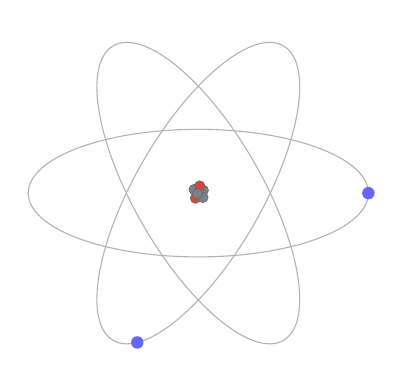
\begin{tikzpicture}[scale=.9,
          p/.style={circle,draw=black!60,fill=proton,minimum size=3.8pt,inner sep=0pt,line width=.2pt},
          n/.style={circle,draw=black!60,fill=neutron,minimum size=3.8pt,inner sep=0pt,line width=.2pt}]
        % electron "cloud"
        \foreach \a in {0,60,120}
        \draw[black!30,rotate=\a] (0,0) ellipse (2.4 and .9);
        \fill[blue!60] (2.4,0) circle (2.5pt);
        \fill[blue!60] ({2.4*cos(200)*cos(60)-.9*sin(200)*sin(60)},{2.4*cos(200)*sin(60)+.9*sin(200)*cos(60)}) circle (2.5pt);
        % nucleus
        \node[p] at (0,0) {};        \node[n] at (.07,.04) {};
        \node[n] at (-.06,.05) {};   \node[p] at (.02,.1) {};
        \node[p] at (-.04,-.07) {};  \node[n] at (.065,-.06) {};
        \node[n] at (-.01,-.01) {};
      \end{tikzpicture}

      {\scriptsize\color{black!50} not to scale}
    \end{column}
    \begin{column}{.55\textwidth}
      \begin{stack}
        \item A \textbf{nucleus} of \textcolor{proton}{protons} ($+$) and \textcolor{neutron}{neutrons} ($0$): the \emph{nucleons}
        \item A cloud of \textcolor{blue!60}{electrons} ($-$) far outside it
        \item Nearly all the mass is in the nucleus
        \item The nucleus is $\sim 1/100{,}000$ the width of the atom: a pea in the middle of a football stadium
      \end{stack}
    \end{column}
  \end{columns}
\end{frame}

%%% --- Forces -------------------------------------------------------

\begin{frame}{What holds a nucleus together?}
  \centering
  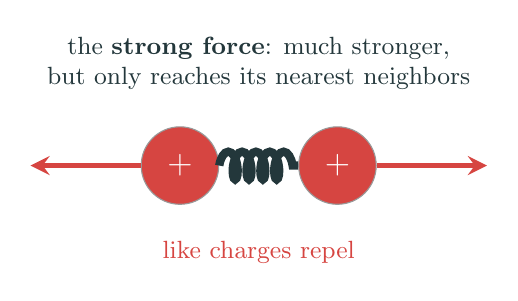
\begin{tikzpicture}[pp/.style={circle,fill=proton,draw=black!40,minimum size=28pt,font=\large\bfseries,text=white}]
    \node[pp] (a) at (-1,0) {$+$};
    \node[pp] (b) at ( 1,0) {$+$};
    \draw[-stealth, line width=2pt, proton] (a.west) -- ++(-1.4,0);
    \draw[-stealth, line width=2pt, proton] (b.east) -- ++( 1.4,0);
    \node[proton, font=\small] at (0,-1.1) {like charges repel};
    \only<2->{
        \draw[accent, line width=3pt, decorate, decoration={coil, aspect=.4, segment length=5pt, amplitude=5pt}]
        (a.east) -- (b.west);
        \node[accent, font=\small, align=center] at (0,1.3) {the \textbf{strong force}: much stronger,\\but only reaches its nearest neighbors};
      }
  \end{tikzpicture}

  \note{Gravity is irrelevant: between two protons it is $\sim10^{36}$ times weaker than the electric force.
    Strong force range $\sim10^{-15}$ m, about one nucleon width.}
\end{frame}

\begin{frame}{\dots\ but in a big nucleus?}
  \begin{columns}[c]
    \begin{column}{.5\textwidth}
      \centering
      \input{fig-bignucleus.tex}
    \end{column}
    \begin{column}{.5\textwidth}
      \only<1>{Pick one proton on the edge.}
      \only<2->{\textcolor{proton}{\textbf{Pushed}} by \emph{every} other proton.}

      \medskip
      \only<3->{\textcolor{accent}{\textbf{Glued}} only to its few neighbors.}

      \bigskip
      \only<4->{\Large The bigger the nucleus, the closer the tug-of-war.}
    \end{column}
  \end{columns}
\end{frame}

%%% --- Binding energy -----------------------------------------------

% Same visual language as "Where the energy comes from": shrinking nucleons = less mass,
% the flash = the missing mass leaving as energy. Not to scale.
\begin{frame}{The missing mass}
  \centering
  \vfill
  \begin{tikzpicture}
    \path (-4,-1.5) rectangle (4,1.5); % fixed bounding box across overlays
    \only<1>{
        \fill[proton]  (-3.2, .8) circle (.3);  \fill[neutron] (-1.4,-.9) circle (.3);
        \fill[neutron] ( 1.5, .9) circle (.3);  \fill[proton]  ( 3.1,-.7) circle (.3);
        \foreach \x/\y in {-3.2/.8, -1.4/-.9, 1.5/.9, 3.1/-.7}
        \draw[-{Stealth[length=5pt]}, black!35] (\x,\y) ++({-\x/7},{-\y/7}) -- ++({-\x/5},{-\y/5});
        \node[font=\small, black!70] at (0,-1.5) {2 protons + 2 neutrons};
      }
    \only<2>{
        \fill[proton] (-.3,.3) circle (.3);  \fill[neutron] (.3,.3) circle (.3);
        \fill[neutron] (-.3,-.3) circle (.3); \fill[proton] (.3,-.3) circle (.3);
        \node[font=\small, black!70] at (0,-1.5) {helium};
      }
    \only<3->{
        \shade[inner color=fissionc!80, outer color=white] (0,0) circle (1.4);
        \foreach \a in {10,30,...,350} \draw[fissionc, line width=1.4pt] (\a:.75) -- (\a:{1.15+.2*mod(\a,40)/20});
        \fill[proton] (-.3,.3) circle (.2);  \fill[neutron] (.3,.3) circle (.2);
        \fill[neutron] (-.3,-.3) circle (.2); \fill[proton] (.3,-.3) circle (.2);
        \draw[black!30, dashed] (-.3,.3) circle (.3) (.3,.3) circle (.3) (-.3,-.3) circle (.3) (.3,-.3) circle (.3);
        \node[font=\small, black!70] at (0,-1.5) {helium};
      }
  \end{tikzpicture}
  \vfill
  \only<3->{Bound together, each nucleon weighs \textbf{less}.\\
      The missing mass, the \textbf{mass defect}, leaves as energy: $E = mc^2$.\\
      {\scriptsize\color{black!50}(shrinking exaggerated)}}

  \note{Helium-4: parts 4.0319 u, nucleus 4.0015 u, so 0.75\% is missing (28.3 MeV): the binding energy.
    This is fusion; it powers the Sun, which loses $\sim$4 million tonnes of mass per second
    (luminosity $3.8\times10^{26}$ W $\div c^2$). Save for the H-bomb in Section 2.}
\end{frame}

\begin{frame}{How tightly bound is each nucleus?}
  \centering
  \begin{tikzpicture}
    \begin{axis}[
        width=.92\textwidth, height=.76\textheight,
        xmin=0, xmax=250, ymin=0, ymax=9.6,
        xlabel={Size of nucleus (number of protons $+$ neutrons)},
        ylabel={Binding energy per nucleon (MeV)},
        axis lines=left, tick style={black!50},
        label style={font=\small}, tick label style={font=\footnotesize},
        clip=false,
      ]
      % Shaded regions (drawn first so the curve sits on top)
      \only<3->{\fill[fusionc, opacity=.18] (axis cs:0,0) rectangle (axis cs:56,9.6);}
      \only<4->{\fill[fissionc, opacity=.18] (axis cs:56,0) rectangle (axis cs:250,9.6);}

      % Nuclide data (AME2020, rounded)
      \addplot[accent, thick, mark=*, mark size=1.1pt] coordinates {
          (1,0) (2,1.112) (3,2.573) (4,7.074) (6,5.332) (7,5.606) (9,6.463)
          (11,6.928) (12,7.680) (14,7.476) (16,7.976) (19,7.779) (20,8.032)
          (23,8.112) (24,8.261) (27,8.332) (28,8.448) (32,8.493) (40,8.551)
          (48,8.723) (52,8.776) (56,8.790) (62,8.795) (64,8.736) (84,8.717)
          (90,8.710) (98,8.635) (120,8.505) (132,8.428) (138,8.393)
          (142,8.346) (158,8.202) (166,8.142) (184,7.930) (195,7.927)
          (208,7.868) (226,7.662) (232,7.615) (235,7.591) (238,7.570)
        };

      \node[font=\scriptsize, anchor=south west] at (axis cs:3,7.2) {helium};
      \node[font=\scriptsize, anchor=south] at (axis cs:235,7.7) {uranium};
      % Peak (nickel-62 is a hair higher per nucleon; "the iron peak" is the usual shorthand)
      \only<2->{
          \draw[black!60, dashed] (axis cs:56,0) -- (axis cs:56,9.6);
          \draw[accent, thick] (axis cs:56,8.79) circle (3pt);
          \node[accent, font=\small, anchor=south west] at (axis cs:58,8.95) {iron: the most tightly bound};
        }
      \only<3->{
          \node[fusionc!70!black, font=\small, align=center] at (axis cs:28,2.6)
          {\textbf{fusion}\\releases\\energy};
          \draw[-stealth, very thick, fusionc!70!black] (axis cs:8,4.4) -- (axis cs:40,6.6);
        }
      \only<4->{
          \node[fissionc!70!black, font=\small, align=center] at (axis cs:150,3.6)
          {\textbf{fission} releases energy};
          \draw[-stealth, very thick, fissionc!70!black] (axis cs:235,6.9) -- (axis cs:150,7.6);
        }
    \end{axis}
  \end{tikzpicture}

  \note{Splitting U-235 (7.6 MeV/nucleon) into fragments like barium + krypton ($\approx$8.5 MeV/nucleon)
    gains $\approx$0.9 MeV $\times$ 235 $\approx$ 200 MeV per fission.
    Chemical reactions rearrange electrons: a few eV per bond. Every conventional bomb is chemistry.}
\end{frame}

% One fission, drawn with real nuclei; see assets/fig-fission-shrink.tex.
\begin{frame}{Where the energy comes from}
  \centering
  \vfill
  \input{fig-fission-shrink.tex}
  \vfill
  \only<2->{Same 236 nucleons, but each one now weighs a little \textbf{less}.\\
      {\scriptsize\color{black!50}(shrinking exaggerated)}}
  \only<3->{\\[.4em] A bomb does this $\sim\!10^{24}$ times.}
  \only<4>{\\[.2em] Hiroshima, all added up: less mass than a \textbf{paperclip}.}

  \note{Nucleons are conserved; mass is not. Mass defect of products minus reactants:
    Ba-141 (1174 MeV) + Kr-92 (783 MeV) $-$ U-235 (1784 MeV) $\approx$ 173 MeV $\approx$ 0.19 u,
    i.e.\ about 1/5 of a nucleon's mass, or 0.08\% per nucleon.
    $\sim$200 MeV is the usual round number once the fragments' later decays are included.
    1 kg of U-235 $\approx 2.6\times10^{24}$ nuclei $\approx$ 17--20 kt, $\approx$ 0.8 g of mass gone.
    Little Boy: $\sim$15 kt $= 6.3\times10^{13}$ J $\div c^2 \approx 0.7$ g converted; a paperclip is $\sim$1 g.}
\end{frame}

%%% --- Energy scale -------------------------------------------------

% xkcd 1162 "Log Scale": the comparison on a linear scale
\begin{frame}[plain]
  \centering
  \vfill
  \maybegraphic[height=.85\textheight,keepaspectratio]{xkcd-1162.png}
  \vfill
  {\scriptsize\color{black!50}\href{https://xkcd.com/1162/}{xkcd.com/1162}\par}
\end{frame}

\begin{frame}{Energy per kilogram}
  \centering
  \begin{tikzpicture}
    \begin{axis}[
        xbar, xmode=log, log origin=infty, bar shift=0pt,
        width=.85\textwidth, height=.7\textheight,
        xmin=0.1, xmax=1e9,
        bar width=10pt,
        symbolic y coords={Phone battery,TNT,Coal,Gasoline,Uranium,Hydrogen},
        ytick={Phone battery,TNT,Coal,Gasoline,Uranium,Hydrogen}, y dir=reverse,
        yticklabels={Phone battery, TNT, Coal, Gasoline,
              {\textcolor{fissionc!85!black}{Uranium \textbf{fission}}},
              {\textcolor{fusionc!85!black}{Hydrogen \textbf{fusion}}}},
        xlabel={Megajoules per kilogram (log scale)},
        axis lines=left, tick style={black!50},
        label style={font=\small}, tick label style={font=\footnotesize},
        enlarge y limits=.12, clip=false,
      ]
      \addplot[fill=neutron, draw=none] coordinates {
          (0.9,Phone battery) (4.2,TNT) (24,Coal) (46,Gasoline)
        };
      \only<2->{
          \addplot[fill=fissionc, draw=none] coordinates {(8.2e7,Uranium)};
          \addplot[fill=fusionc, draw=none] coordinates {(3.4e8,Hydrogen)};}
      \only<3->{
          \node[white, font=\footnotesize\bfseries, anchor=west] at (axis cs:20,Uranium) {$\approx$ 20 million $\times$ TNT};
        }
    \end{axis}
  \end{tikzpicture}

  \note{Uranium = U-235 fission; hydrogen = deuterium--tritium fusion.
    1 kg of U-235, fully fissioned $\approx$ 20 kilotons of TNT.
    Hiroshima: $\sim$15 kt, from less than 1 kg actually fissioning (of 64 kg on board).}
\end{frame}

%%% --- Isotopes & stability ------------------------------------------

\begin{frame}{Isotopes}
  \centering
  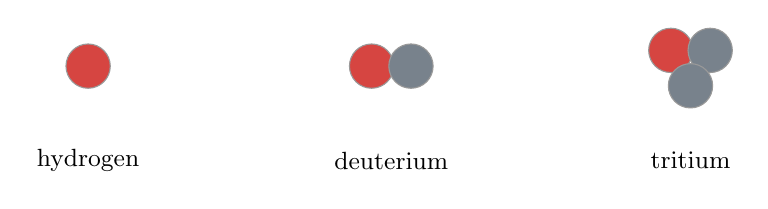
\begin{tikzpicture}[
      pp/.style={circle,fill=proton,draw=black!40,minimum size=16pt,inner sep=0pt},
      nn/.style={circle,fill=neutron,draw=black!40,minimum size=16pt,inner sep=0pt},
      lbl/.style={font=\small, align=center}]
    \node[pp] at (0,0) {};
    \node[lbl] at (0,-1.2) {hydrogen};
    \onslide<2->{
        \node[pp] at (3.6,0) {}; \node[nn] at (4.1,0) {};
        \node[lbl] at (3.85,-1.2) {deuterium};
      }
    \onslide<3->{
        \node[pp] at (7.4,.2) {}; \node[nn] at (7.9,.2) {}; \node[nn] at (7.65,-.25) {};
        \node[lbl] at (7.65,-1.2) {tritium};
      }
  \end{tikzpicture}

  \vspace{1.5em}
  \onslide<4->{Same element, different number of \textcolor{neutron}{\textbf{neutrons}}.}

  \smallskip
  \onslide<5->{Chemically identical. \emph{Nuclearly} very different.}
\end{frame}

\begin{frame}{Natural uranium}
  \centering
  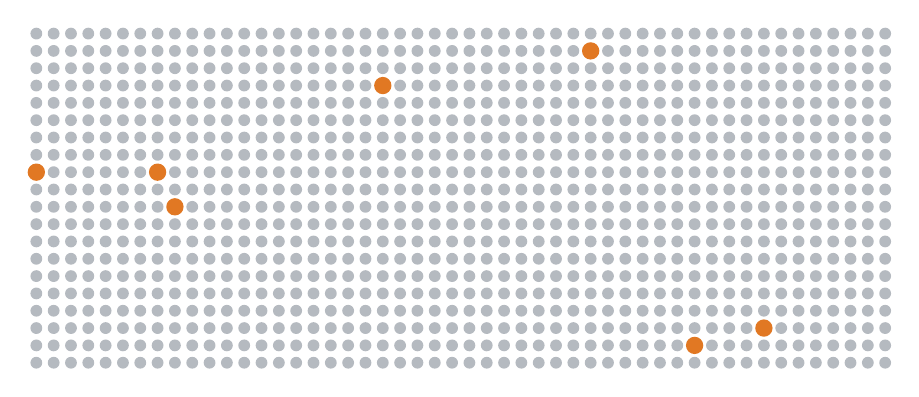
\begin{tikzpicture}
    \foreach \i in {0,...,49} \foreach \j in {0,...,19}
    \fill[neutron!55] (\i*.22, -\j*.22) circle (.075);
    \only<2->{
        \fill[fissionc] (1.54,-1.76) circle (.11);
        \fill[fissionc] (0.00,-1.76) circle (.11);
        \fill[fissionc] (8.36,-3.96) circle (.11);
        \fill[fissionc] (9.24,-3.74) circle (.11);
        \fill[fissionc] (1.76,-2.20) circle (.11);
        \fill[fissionc] (7.04,-0.22) circle (.11);
        \fill[fissionc] (4.40,-0.66) circle (.11);
      }
  \end{tikzpicture}

  \vspace{1em}
  1{,}000 uranium atoms.
  \onslide<2->{Only \textcolor{fissionc}{\textbf{7}} are U-235, the kind that splits easily.}

  \note{Natural uranium: 99.3\% U-238, 0.7\% U-235. Concentrating the U-235 is \emph{enrichment}: Section 2.}
\end{frame}

\begin{frame}{The valley of stability}
  \centering
  \begin{tikzpicture}
    \begin{axis}[
        width=.8\textwidth, height=.8\textheight,
        xmin=0, xmax=105, ymin=0, ymax=165,
        xlabel={Protons}, ylabel={Neutrons},
        axis lines=left, tick style={black!50},
        label style={font=\small}, tick label style={font=\footnotesize},
        clip=false,
      ]
      \addplot[black!35, dashed, domain=0:100] {x};
      \node[black!50, font=\scriptsize, anchor=west] at (axis cs:100,100) {equal numbers};
      % approximate line of stability: Z = A / (1.98 + 0.0155 A^{2/3})
      \addplot[accent, line width=9pt, opacity=.25, domain=2:265, samples=80]
      ({x/(1.98+0.0155*x^(2/3))}, {x - x/(1.98+0.0155*x^(2/3))});
      \node[accent, font=\small, rotate=50] at (axis cs:52,80) {stable};
      \only<2->{
          \node[font=\small, black!70, align=center] at (axis cs:22,120) {too many\\neutrons};
          \node[font=\small, black!70, align=center] at (axis cs:85,40) {too many\\protons};
        }
      \only<3->{
          \addplot[only marks, mark=*, mark size=2pt, fissionc] coordinates {(92,143) (92,146)};
          \node[font=\small, anchor=west] at (axis cs:93,144) {uranium};
        }
    \end{axis}
  \end{tikzpicture}

  \note{Heavy nuclei need extra neutrons: strong-force glue without the repulsion.
    Off the band $\Rightarrow$ unstable. Nothing heavier than lead-208 is truly stable.}
\end{frame}

%%% --- Radioactivity --------------------------------------------------

\begin{frame}{Radioactivity}
  \centering
  Unstable nuclei \textbf{decay}, throwing something out.

  \bigskip
  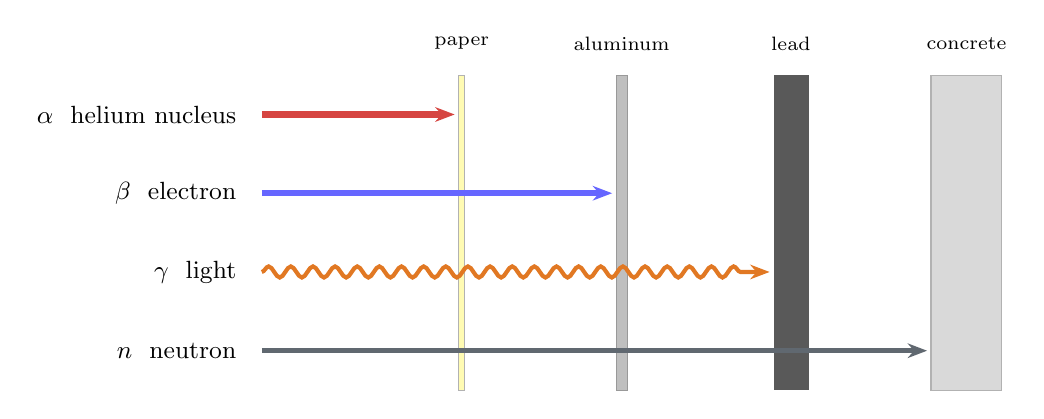
\begin{tikzpicture}[lbl/.style={font=\small, anchor=east, align=right}]
    % barriers
    \fill[yellow!30!white, draw=black!30] (3,-2) rectangle (3.08,2);
    \fill[black!25, draw=black!40]        (5,-2) rectangle (5.15,2);
    \fill[black!65]                        (7,-2) rectangle (7.45,2);
    \fill[black!15, draw=black!30]         (9,-2) rectangle (9.9,2);
    \node[font=\scriptsize, align=center] at (3.04,2.4)  {paper};
    \node[font=\scriptsize, align=center] at (5.07,2.4)  {aluminum};
    \node[font=\scriptsize, align=center] at (7.22,2.4)  {lead};
    \node[font=\scriptsize, align=center] at (9.45,2.4)  {concrete};
    % rays
    \onslide<2->{\node[lbl] at (.3,1.5) {$\alpha$\ \ helium nucleus};
        \draw[-{Stealth[length=7pt]}, line width=2.5pt, proton] (.5,1.5) -- (2.95,1.5);}
    \onslide<3->{\node[lbl] at (.3,.5) {$\beta$\ \ electron};
        \draw[-{Stealth[length=7pt]}, line width=2pt, blue!60] (.5,.5) -- (4.95,.5);}
    \onslide<4->{\node[lbl] at (.3,-.5) {$\gamma$\ \ light};
        \draw[-{Stealth[length=7pt]}, line width=1.5pt, fissionc, decorate,
          decoration={snake, amplitude=2pt, segment length=8pt, post length=7pt}] (.5,-.5) -- (6.95,-.5);}
    \onslide<5->{\node[lbl] at (.3,-1.5) {$n$\ \ neutron};
        \draw[-{Stealth[length=7pt]}, line width=2pt, neutron!80!black] (.5,-1.5) -- (8.95,-1.5);}
  \end{tikzpicture}
\end{frame}

\begin{frame}{Half-life}
  \begin{columns}[c]
    \begin{column}{.45\textwidth}
      \centering
      \input{fig-halflife-sim.tex}
    \end{column}
    \begin{column}{.55\textwidth}
      \only<1>{64 radioactive atoms.\\[.5em] Each one decays at a random moment.}
      \only<2->{After each \textbf{half-life}, half of what's left is gone.}

      \bigskip
      \Huge
      \only<1>{64}\only<2>{32}\only<3>{16}\only<4>{8}\only<5>{4}\only<6>{2}
      \normalsize
      \only<2->{\ \ remaining}
    \end{column}
  \end{columns}
\end{frame}

\begin{frame}{How long is a half-life?}
  \centering
  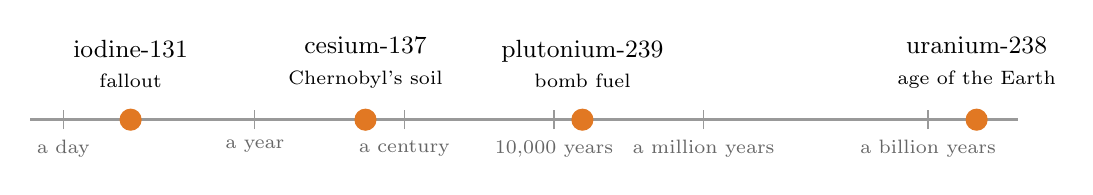
\begin{tikzpicture}[x=.95cm]
    % log10(years) + 3, so 0 = a millennium^{-1}
    \draw[black!40, line width=1pt] (0,0) -- (13.2,0);
    \foreach \x/\l in {.44/a day, 3/a year, 5/a century, 7/10{,}000 years, 9/a million years, 12/a billion years}
      { \draw[black!40] (\x,-.12) -- (\x,.12); \node[font=\scriptsize, black!60, below=4pt] at (\x,0) {\l}; }
    \onslide<2->{\fill[fissionc] (1.34,0) circle (4pt);
        \node[font=\small, align=center, above=8pt] at (1.34,0) {iodine-131\\{\scriptsize fallout}};}
    \onslide<3->{\fill[fissionc] (4.48,0) circle (4pt);
        \node[font=\small, align=center, above=8pt] at (4.48,0) {cesium-137\\{\scriptsize Chernobyl's soil}};}
    \onslide<4->{\fill[fissionc] (7.38,0) circle (4pt);
        \node[font=\small, align=center, above=8pt] at (7.38,0) {plutonium-239\\{\scriptsize bomb fuel}};}
    \onslide<5->{\fill[fissionc] (12.65,0) circle (4pt);
        \node[font=\small, align=center, above=8pt] at (12.65,0) {uranium-238\\{\scriptsize age of the Earth}};}
  \end{tikzpicture}

  \note{I-131: 8 days. Cs-137: 30 years. Pu-239: 24{,}000 years. U-238: 4.5 billion years.}
\end{frame}

\begin{frame}{What radiation looks like}
  \begin{columns}[c]
    \begin{column}{.6\textwidth}\centering
      % photos/cloudchamber-alt.jpg is two photos side by side (1920x1445 px); show only the left one
      \IfFileExists{photos/cloudchamber-alt.jpg}{%
        \begin{tikzpicture}
          \clip (0,0) rectangle (4.4,6.62);
          \node[anchor=south west, inner sep=0] at (0,0) {\includegraphics[width=8.8cm]{photos/cloudchamber-alt.jpg}};
        \end{tikzpicture}}{\maybegraphic{photos/cloudchamber-alt.jpg}}
    \end{column}
    \begin{column}{.4\textwidth}
      A cloud chamber near a radioactive source: every streak is \textbf{one particle}.

      \medskip
      \onslide<2->{Each streak is a trail of thousands of smashed molecules.}

      \medskip
      \onslide<3->{Now picture that trail going through your cells.}
    \end{column}
  \end{columns}
  \note{Cloud chamber: supersaturated alcohol vapor condenses on the ions a charged particle leaves behind.
    A decay particle carries $\sim$1 MeV; breaking a chemical bond takes a few eV, so one particle can ionize
    tens of thousands of molecules. Some of those are DNA.}
\end{frame}

\begin{frame}{Seeing single atoms decay}
  \begin{columns}[c]
    \begin{column}{.55\textwidth}\centering
      \maybegraphic[width=\textwidth,height=.75\textheight,keepaspectratio]{photos/radiumdial.jpg}
    \end{column}
    \begin{column}{.45\textwidth}
      Radium paint glows in the dark.

      \medskip
      \onslide<2->{Each tiny flash is \textbf{one atom} decaying: its alpha particle hits a crystal and makes light.}

      \medskip
      \onslide<3->{The same particles, inside a body, hit cells instead.}
    \end{column}
  \end{columns}
  \note{Radium dials: radium mixed with zinc sulfide; each alpha particle makes a scintillation (Crookes' spinthariscope,
    1903, let you watch individual flashes through a magnifier). The Radium Girls (1920s dial painters) licked their
    brushes to a point (``lip, dip, paint''); radium behaves like calcium and settles in bone, so many later developed
    anemia, bone damage and cancer. Their lawsuits helped create occupational radiation-safety rules.
    Big dose fast: cells die (radiation sickness). Small dose over time: mis-repaired DNA, higher odds of cancer.}
\end{frame}

%%% --- Handoff to Section 2 -----------------------------------------

\begin{frame}{Why neutrons?}
  \centering
  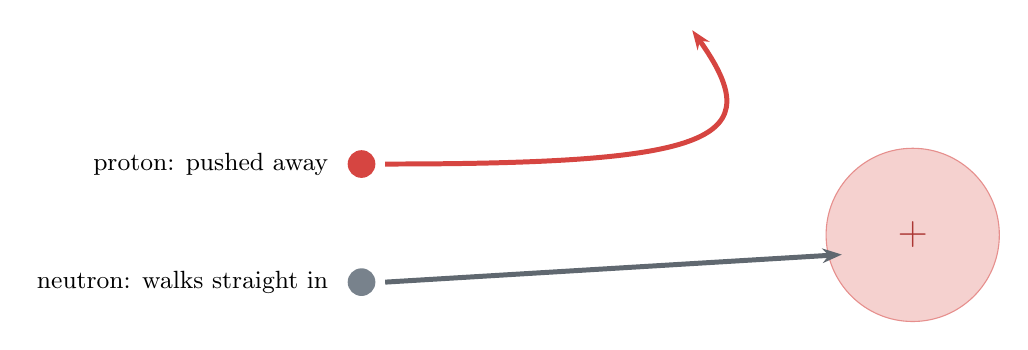
\begin{tikzpicture}
    \fill[proton!25, draw=proton!60] (7,0) circle (1.1);
    \node[proton!80!black, font=\Large] at (7,0) {$+$};
    \onslide<1->{
        \fill[proton] (0,.9) circle (5pt);
        \draw[-{Stealth[length=7pt]}, line width=1.8pt, proton]
        (.3,.9) .. controls (4.5,.9) and (5.2,1.2) .. (4.2,2.6);
        \node[font=\small, anchor=east] at (-.3,.9) {proton: pushed away};
      }
    \onslide<2->{
        \fill[neutron] (0,-.6) circle (5pt);
        \draw[-{Stealth[length=7pt]}, line width=1.8pt, neutron!80!black] (.3,-.6) -- (6.1,-.25);
        \node[font=\small, anchor=east] at (-.3,-.6) {neutron: walks straight in};
      }
  \end{tikzpicture}
\end{frame}

\begin{frame}{Fission}
  \centering
  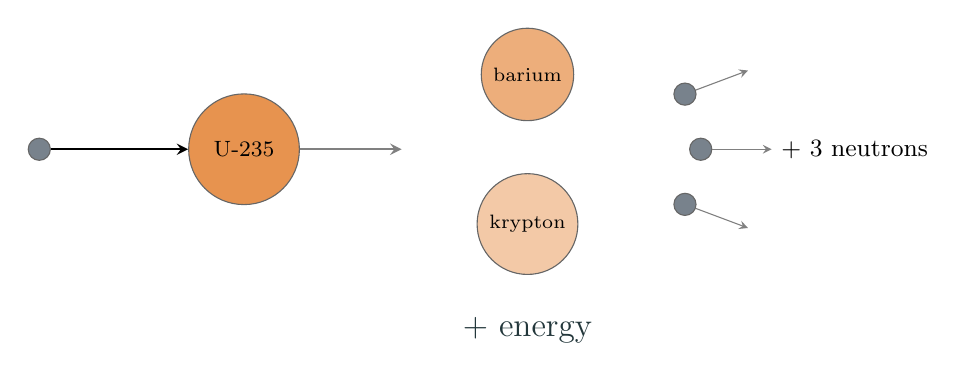
\begin{tikzpicture}[
      n/.style={circle,draw=black!60,fill=neutron,minimum size=8pt,inner sep=0pt}]
    \node[n] (n0) at (0,0) {};
    \node[circle, draw=black!60, fill=fissionc!80, minimum size=40pt, font=\footnotesize] (u) at (2.6,0) {U-235};
    \draw[-stealth, thick] (n0) -- (u);
    \only<2->{
        \draw[-stealth, thick, black!50] (u) -- (4.6,0);
        \node[circle, draw=black!60, fill=fissionc!60, minimum size=30pt, font=\scriptsize] at (6.2,.95) {barium};
        \node[circle, draw=black!60, fill=fissionc!40, minimum size=26pt, font=\scriptsize] at (6.2,-.95) {krypton};
        \node[font=\large, accent] at (6.2,-2.3) {+ energy};
      }
    \only<2->{
        \node[n] (a) at (8.2,.7) {};  \node[n] (b) at (8.4,0) {};  \node[n] (c) at (8.2,-.7) {};
        \draw[-stealth, black!50] (a) -- ++(.8,.3);
        \draw[-stealth, black!50] (b) -- ++(.9,0);
        \draw[-stealth, black!50] (c) -- ++(.8,-.3);
        \node[font=\small, anchor=west] at (9.3,0) {+ 3 neutrons};
      }
  \end{tikzpicture}

  \vspace{1em}
  \only<3>{\Large What if each of those hits \emph{another} U-235?}

  \note{n + U-235 $\to$ Ba-141 + Kr-92 + 3n + $\approx$200 MeV.}
\end{frame}

% Chain reaction: one generation per click; see assets/fig-chain-reaction.tex.
% Chain reaction: Monte Carlo, one generation per click; see assets/gen/chain_reaction.py (seed 6).
\begin{frame}{Chain reaction}
  \begin{columns}[c]
    \begin{column}{.55\textwidth}
      \centering
      \input{fig-chain-reaction.tex}
    \end{column}
    \begin{column}{.45\textwidth}
      {\Huge \only<1>{1}\only<2>{2}\only<3>{3}\only<4>{5}\only<5>{9}\only<6->{16}}
      \ \ fissions in generation
      \only<1>{1}\only<2>{2}\only<3>{3}\only<4>{4}\only<5>{5}\only<6->{6}

      \bigskip
      \onslide<3->{\textcolor{black!50}{Some neutrons \textbf{escape} the lump; some are \textbf{captured} ($\times$).}}

      \bigskip
      \onslide<6->{Each generation $\approx$ 1.7 times the last:\\ \textbf{$k \approx 1.7$}.}

      \bigskip
      \onslide<7->{About \textbf{80 generations}:\\
          $\sim\!10^{24}$ fissions, in under a \textbf{microsecond}.}
    \end{column}
  \end{columns}

  \note{A real Monte Carlo (in 2D): each fission emits 2 or 3 neutrons (2.4 on average) in random directions; each
    neutron flies an exponentially distributed distance before it interacts; it escapes if it leaves the lump, is
    captured 15\% of the time, otherwise splits the nearest nucleus. Fissions per generation: 1, 2, 3, 5, 9, 16.
    Not to scale: real nuclei are far smaller and farther apart, and a neutron passes millions of atoms between hits.
    Other seeds fizzle (e.g.\ seed 5 dies after 2 generations): that's a sub-critical lump.
    A generation takes $\sim$10 ns in a bomb, so 80 generations $\approx$ 1 $\mu$s; $1.7^{80}$ and $2^{80}$ are both astronomically large.}
\end{frame}

% % CP-1. Data: Rhodes, The Making of the Atomic Bomb, pp. 434-440 (from Fermi's own chart).
% \begin{frame}{Chicago, 2 December 1942}
%   \begin{columns}[c]
%     \begin{column}{.58\textwidth}\centering
%       \begin{tikzpicture}
%         \begin{axis}[width=\textwidth, height=.7\textheight, xmin=0, xmax=60, ymin=0, ymax=420,
%             axis lines=left, tick style={black!50}, xlabel={Layers of graphite and uranium},
%             ylabel={Fermi's countdown}, label style={font=\small}, tick label style={font=\footnotesize}, clip=false]
%           \only<1->{\addplot[only marks, mark=*, mark size=2.2pt, fissionc] coordinates {(15,390)};}
%           \only<2->{\addplot[only marks, mark=*, mark size=2.2pt, fissionc] coordinates {(19,320) (25,270)};}
%           \only<3->{\addplot[only marks, mark=*, mark size=2.2pt, fissionc] coordinates {(36,149)};}
%           \only<4->{\draw[black!50, dashed, thick] (axis cs:36,149) -- (axis cs:56.5,0);
%                     \node[font=\scriptsize, black!60, anchor=south west] at (axis cs:46,80) {Fermi's prediction};}
%           \only<5->{\node[fissionc!80!black, font=\Large] at (axis cs:57,0) {$\star$};
%                     \node[font=\scriptsize\bfseries, anchor=south] at (axis cs:57,12) {layer 57};}
%         \end{axis}
%       \end{tikzpicture}
%     \end{column}
%     \begin{column}{.42\textwidth}
%       Every layer: more uranium, fewer neutrons escape.

%       \medskip
%       \onslide<4->{The countdown hits zero when $k = 1$: each generation exactly replaces the last.}

%       \medskip
%       \onslide<5->{$k = 1.0006$.\\ The first self-sustaining chain reaction.}

%       \medskip
%       \onslide<6->{It ran 4.5 minutes, at half a watt.}
%     \end{column}
%   \end{columns}

%   \note{Countdown = (radius of the pile)$^2$ $\div$ neutron activity measured with indium foils; it falls to zero at criticality.
%     Rhodes: 390 at layer 15, 320 at layer 19, 270 at layer 25, 149 at layer 36; Fermi predicted zero between layers 56 and 57.
%     At $k = 1.0006$ the intensity doubled every two minutes; left alone for 90 minutes it would have reached a million kilowatts.
%     ``ZIP in!'' at 3:53 pm. Contrast: a reactor sits at $k = 1$; a bomb needs $k$ well above 1 and must get there in a microsecond.
%     Fermi's first lattice at Columbia (1941) had $k = 0.87$.}
% \end{frame}


%%% ===============================================================
\section{Nuclear Weapons}
%%% ===============================================================

\definecolor{icbmc}{RGB}{190,60,50}    % land-based missiles
\definecolor{slbmc}{RGB}{40,90,160}    % submarine-launched missiles
\definecolor{bomberc}{RGB}{95,95,95}   % aircraft

%%% --- The map -------------------------------------------------------

\begin{frame}{Where the weapons are}
  \centering
  \input{fig-world-map.tex}

  \vspace{.3em}
  \only<1>{\small $\sim$12{,}000 warheads, nine countries.}
  \only<2->{\scriptsize
      \tikz\fill[icbmc] (0,0) -- (.2,0) -- (.1,.18) -- cycle;\ land missiles \quad
      \tikz\fill[slbmc] (0,0) circle (.08);\ submarine bases \quad
      \tikz\fill[bomberc] (0,0) rectangle (.15,.15);\ bombers / aircraft \quad
      \tikz{\draw[black!70] (0,0) circle (.1); \node[font=\tiny\bfseries] at (0,0) {?};}\ sites undisclosed}

  \note{FAS ``Status of World Nuclear Forces'' 2026, total inventories: Russia 5{,}420; US 5{,}042; China 620;
    France 370; UK 225; India 190; Pakistan 170; Israel 90; North Korea 60. Total $\approx$ 12{,}187.
    Squares in Europe: $\sim$100 US B61 bombs at bases in Belgium, Germany, Italy, the Netherlands, Turkey
    (nuclear sharing). Russian/Chinese sites are marked at the garrison town; locations approximate.}
\end{frame}

%%% --- Fission weapons --------------------------------------------------

% \begin{frame}{Weapons-grade uranium}
%   \centering
%   \begin{tikzpicture}
%     \foreach \i in {0,...,49} \foreach \j in {0,...,19}
%     \fill[fissionc] (\i*.22, -\j*.22) circle (.075);
%     \foreach \p in {{(2.86,0.00)}, {(3.30,0.00)}, {(6.38,0.00)}, {(6.82,0.00)}, {(7.92,0.00)}, {(9.46,0.00)}, {(3.30,-0.22)}, {(3.74,-0.22)}, {(10.78,-0.22)}, {(7.26,-0.44)}, {(8.14,-0.44)}, {(8.58,-0.44)}, {(0.88,-0.66)}, {(1.10,-0.66)}, {(2.86,-0.66)}, {(10.12,-0.66)}, {(4.84,-0.88)}, {(8.14,-0.88)}, {(8.58,-0.88)}, {(9.46,-0.88)}, {(3.08,-1.10)}, {(3.30,-1.10)}, {(5.50,-1.10)}, {(7.92,-1.10)}, {(1.76,-1.32)}, {(9.68,-1.32)}, {(1.98,-1.54)}, {(5.28,-1.54)}, {(6.16,-1.54)}, {(9.90,-1.54)}, {(10.12,-1.54)}, {(10.78,-1.54)}, {(0.88,-1.76)}, {(1.32,-1.76)}, {(3.74,-1.76)}, {(6.82,-1.76)}, {(8.14,-1.76)}, {(10.12,-1.76)}, {(1.10,-1.98)}, {(6.60,-1.98)}, {(6.82,-1.98)}, {(7.48,-1.98)}, {(7.70,-1.98)}, {(8.14,-1.98)}, {(1.32,-2.20)}, {(4.18,-2.20)}, {(7.70,-2.20)}, {(10.12,-2.20)}, {(0.66,-2.42)}, {(1.54,-2.42)}, {(2.64,-2.42)}, {(3.08,-2.42)}, {(8.14,-2.42)}, {(8.80,-2.42)}, {(9.68,-2.42)}, {(10.56,-2.42)}, {(10.78,-2.42)}, {(1.10,-2.64)}, {(1.32,-2.64)}, {(1.98,-2.64)}, {(3.96,-2.64)}, {(4.40,-2.64)}, {(8.80,-2.64)}, {(9.02,-2.64)}, {(0.00,-2.86)}, {(0.88,-2.86)}, {(8.14,-2.86)}, {(8.36,-2.86)}, {(10.56,-2.86)}, {(2.64,-3.08)}, {(6.82,-3.08)}, {(7.48,-3.08)}, {(7.92,-3.08)}, {(9.90,-3.08)}, {(1.98,-3.30)}, {(5.72,-3.30)}, {(9.90,-3.30)}, {(10.34,-3.30)}, {(10.56,-3.30)}, {(1.54,-3.52)}, {(4.40,-3.52)}, {(9.46,-3.52)}, {(0.66,-3.74)}, {(1.32,-3.74)}, {(1.54,-3.74)}, {(5.50,-3.74)}, {(5.72,-3.74)}, {(6.82,-3.74)}, {(7.92,-3.74)}, {(8.36,-3.74)}, {(10.78,-3.74)}, {(6.60,-3.96)}, {(8.14,-3.96)}, {(9.24,-3.96)}, {(9.46,-3.96)}, {(10.56,-3.96)}, {(0.66,-4.18)}, {(2.20,-4.18)}, {(4.18,-4.18)}, {(8.36,-4.18)}} \fill[neutron!55] \p circle (.075);
%   \end{tikzpicture}

%   \vspace{1em}
%   Natural uranium: 7 in 1{,}000 split easily. A bomb needs \textbf{900}.

%   \note{Enrichment from 0.7\% to $\sim$90\% U-235 is the hard, slow, industrial part, and the part
%     inspectors watch (NPT/IAEA, Section 3). Plutonium is the other route: made in reactors.}
% \end{frame}

\begin{frame}{Fission bomb: implosion}
  \begin{columns}[c]
    \begin{column}{.5\textwidth}
      \centering
      \begin{tikzpicture}[scale=.9]
        \foreach \a in {0,30,...,330} {
            \fill[black!45, draw=white, line width=1pt] (\a:1.1) arc[start angle=\a, end angle=\a+30, radius=1.1]
            -- (\a+30:1.8) arc[start angle=\a+30, end angle=\a, radius=1.8] -- cycle;
          }
        \only<1>{\fill[fissionc] (0,0) circle (.6);}
        \only<2->{\fill[fissionc] (0,0) circle (.36);
            \foreach \a in {0,45,...,315} \draw[-{Stealth[length=5pt]}, thick, black!70] (\a:2.2) -- (\a:1.25);}
        \only<3->{\shade[inner color=yellow!60, outer color=white, opacity=.9] (0,0) circle (1.2);}
        \node[font=\scriptsize, black!70] at (0,-2.2) {explosive shell};
      \end{tikzpicture}

      \vspace{.4em}
      \small
      \only<1>{A ball of plutonium, too spread out.}
      \only<2->{Squeeze it from every side at once: \textbf{critical}.}
    \end{column}
    \begin{column}{.5\textwidth}
      \centering
      \only<4->{\maybegraphic[width=\textwidth]{photos/trinity.jpg}\\
          {\scriptsize\color{black!60} Trinity, New Mexico, 16 July 1945, 0.016 s after detonation.}}
    \end{column}
  \end{columns}

  \note{Trinity: first nuclear explosion, $\approx$25 kt. Same design as Fat Man (Nagasaki, 9 Aug 1945, $\approx$21 kt).
    Plutonium needs implosion: a gun is too slow for it.}
\end{frame}

\begin{frame}{Fission bomb: the gun}
  \begin{columns}[c]
    \begin{column}{.5\textwidth}
      \centering
      \begin{tikzpicture}[scale=.85, lbl/.style={font=\scriptsize, black!70, align=center}]
        \draw[rounded corners=10pt, black!50, thick] (0,0) rectangle (7,1.6);
        \fill[black!45] (.3,.5) rectangle (.95,1.1);
        \node[lbl, below] at (.62,0) {explosive};
        \draw[black!40] (1,.5) -- (5,.5) (1,1.1) -- (5,1.1);
        % target
        \fill[fissionc] (5,.25) rectangle (6.25,.5);  \fill[fissionc] (5,1.1) rectangle (6.25,1.35);
        \fill[fissionc] (6,.5) rectangle (6.25,1.1);
        \node[lbl, below] at (5.6,0) {uranium};
        % bullet
        \only<1>{\fill[fissionc!55, draw=fissionc!70!black] (1,.55) rectangle (2,1.05); \node[lbl, below] at (2.3,0) {uranium};
            % escaping neutrons (as in the chain-reaction frame): dots leaving each piece's edge
            \foreach \x/\y/\dx/\dy in {1.3/1.25/-.15/.45, 1.75/1.25/.15/.45, 1.5/.35/0/-.45,
                5.3/1.5/-.15/.45, 5.9/1.5/.15/.45, 5.6/.1/0/-.45, 6.45/.8/.45/0} {
                \fill[neutron] (\x,\y) circle (.06);
                \draw[-{Stealth[length=3pt]}, black!40] (\x,\y) ++(\dx/4,\dy/4) -- ++(\dx,\dy);
              }
            \node[font=\scriptsize, black!50, anchor=west] at (2.3,1.9) {neutrons escape};}
        \only<2->{\fill[fissionc!55, draw=fissionc!70!black] (5,.55) rectangle (6,1.05);
            \draw[-{Stealth[length=6pt]}, very thick, black!60] (1.2,.8) -- (4.8,.8);}
        \only<3->{\shade[inner color=yellow!60, outer color=white, opacity=.9] (5.6,.8) circle (1);}
      \end{tikzpicture}

      \vspace{.6em}
      \small
      \only<1>{Two pieces, each too small: neutrons escape.}
      \only<2->{Fire one into the other: suddenly \textbf{critical}.}
    \end{column}
    \begin{column}{.5\textwidth}
      \centering
      \only<4->{\maybegraphic[height=.72\textheight]{photos/hiroshima.jpg}\\
          {\scriptsize\color{black!60} Hiroshima, 6 August 1945. $\sim$15 kilotons.}}
    \end{column}
  \end{columns}

  \note{Little Boy: 64 kg of highly enriched uranium; less than 1 kg fissioned. Killed $\sim$70{,}000--140{,}000 by the end of 1945.
    Critical mass: the chain reaction's escaping neutrons from Section 1.}
\end{frame}


%%% --- Fusion weapons ---------------------------------------------------

\begin{frame}{Fusion bomb: two stages}
  \begin{columns}[c]
    \begin{column}{.5\textwidth}
      \centering
      \begin{tikzpicture}[scale=.85, lbl/.style={font=\scriptsize, black!70, align=center}]
        \draw[rounded corners=12pt, black!50, thick] (0,0) rectangle (7,2.2);
        % primary
        \fill[black!45] (1.2,1.1) circle (.62); \fill[fissionc] (1.2,1.1) circle (.3);
        \node[lbl, below] at (1.2,0) {fission\\primary};
        % secondary
        \only<-2>{\fill[fusionc!70, rounded corners=4pt] (3,.45) rectangle (6.6,1.75);
            \fill[fissionc] (3.2,1.0) rectangle (6.4,1.2);}
        \node[lbl, below] at (4.8,0) {fusion\\secondary};
        \only<2->{\shade[inner color=yellow!60, outer color=white, opacity=.9] (1.2,1.1) circle (.75);
            \foreach \y in {.2,2.0} \draw[-{Stealth[length=5pt]}, fissionc!80!black, thick, decorate,
              decoration={snake, amplitude=1.5pt, segment length=6pt, post length=5pt}] (1.9,\y) -- (6.7,\y);}
        \only<3->{\fill[fusionc!70, rounded corners=3pt] (3.1,.75) rectangle (6.5,1.45);
            \fill[fissionc] (3.2,1.03) rectangle (6.4,1.17);
            \foreach \x in {3.5,4.5,5.5,6.2} \draw[-{Stealth[length=4pt]}, black!70] (\x,1.75) -- (\x,1.5) (\x,.45) -- (\x,.7);}
        \only<4->{\shade[inner color=yellow!70, outer color=white, opacity=.95] (4.8,1.1) ellipse (2.2 and 1.2);}
      \end{tikzpicture}

      \vspace{.4em}
      \small
      \only<1>{An atomic bomb is just the \textbf{trigger}.}
      \only<2>{Its radiation floods the case\dots}
      \only<3>{\dots\ and crushes the fusion fuel.}
      \only<4->{No upper limit on size.}
    \end{column}
    \begin{column}{.5\textwidth}
      \centering
      \only<5->{\maybegraphic[width=\textwidth]{photos/castlebravo.jpg}\\
          {\scriptsize\color{black!60} Castle Bravo, Bikini Atoll, 1 March 1954. 15 megatons: 1{,}000 Hiroshimas.}}
    \end{column}
  \end{columns}

  \note{The Teller--Ulam two-stage design (public, schematic level only). Castle Bravo was expected to yield 6 Mt
    and gave 15: lithium-7 in the fuel turned out to react too. Fallout reached Rongelap Atoll and the crew of
    the Japanese fishing boat \emph{Lucky Dragon No.\ 5}. The radiation/half-life material from Section 1 pays off here.}
\end{frame}

\begin{frame}{Tsar Bomba}
  \begin{columns}[c]
    \begin{column}{.55\textwidth}
      \centering
      \only<1>{\maybegraphic[width=\textwidth]{photos/tsarbomba-casing.jpg}\\
          {\scriptsize\color{black!60} The casing, now in a museum in Sarov.}}
      \only<2->{\maybegraphic[width=\textwidth]{photos/tsarbomba.jpg}\\
          {\scriptsize\color{black!60} Novaya Zemlya, 30 October 1961.}}
    \end{column}
    \begin{column}{.45\textwidth}
      \onslide<2->{{\Huge 50 megatons}}

      \medskip
      \onslide<3->{$\approx$ \textbf{3{,}300} Hiroshimas.}

      \medskip
      \onslide<4->{One of its designers: \textbf{Andrei Sakharov}.}
    \end{column}
  \end{columns}

  \note{Novaya Zemlya, 30 Oct 1961. Designed for 100 Mt; the uranium tamper was swapped for lead to halve the
    yield (and the fallout). Sakharov later estimated $\sim$10{,}000 eventual deaths per megaton of
    atmospheric testing (materials/sgs01sakharov.pdf) and became a dissident: bridge to Section 3 and the test ban.}
\end{frame}

%%% --- Delivery: the triad -------------------------------------------

\begin{frame}{How to deliver it: the triad}
  \centering
  \begin{columns}[t]
    \begin{column}{.32\textwidth}\centering
      \maybegraphic[width=\textwidth,height=.42\textheight,keepaspectratio]{photos/minuteman.jpg}\\[.3em]
      \textcolor{icbmc}{\textbf{Land}}\\ {\small missiles in silos}
    \end{column}
    \begin{column}{.32\textwidth}\centering
      \onslide<2->{\maybegraphic[width=\textwidth,height=.42\textheight,keepaspectratio]{photos/trident.jpg}\\[.3em]
          \textcolor{slbmc}{\textbf{Sea}}\\ {\small missiles on submarines}}
    \end{column}
    \begin{column}{.32\textwidth}\centering
      \onslide<3->{\maybegraphic[width=\textwidth,height=.42\textheight,keepaspectratio]{photos/b52.jpg}\\[.3em]
          \textcolor{bomberc}{\textbf{Air}}\\ {\small bombers}}
    \end{column}
  \end{columns}

  \vspace{1em}
  \onslide<4->{Why three?}
\end{frame}

\begin{frame}{Classifying the triad}
  \centering
  \begin{tikzpicture}[x=1cm, y=1cm, wpn/.style={font=\small\bfseries, align=center}]
    \draw[black!30] (4,0) -- (4,5.2) (0,2.6) -- (8,2.6);
    \draw[-{Stealth[length=6pt]}, thick, black!60] (0,0) -- (8.3,0)
    node[below left, font=\small, black] {can destroy the enemy's weapons};
    \draw[-{Stealth[length=6pt]}, thick, black!60] (0,0) -- (0,5.5)
    node[above, font=\small, black] {survives a first strike};
    \only<2->{\node[wpn, slbmc] at (2,4.2) {submarine\\missiles};}
    \only<3->{\node[wpn, icbmc] at (6,1.3) {missiles\\in silos};}
    \only<4->{\node[wpn, bomberc] at (2.3,1.1) {bombers\\on the ground};
        \draw[-{Stealth[length=5pt]}, bomberc, dashed] (2.3,1.65) -- (2.3,3.05)
        node[above, font=\scriptsize\bfseries, bomberc] {airborne (and recallable)};}
  \end{tikzpicture}

  \note{Survivability: can it ride out a surprise attack (second strike)? Counterforce: is it accurate and fast
    enough to destroy the other side's weapons? Submarines are hard to find, so they survive. Silos are fixed
    and targetable, but their missiles are fast and accurate. Bombers are vulnerable on the ground, survivable
    once airborne, and the only leg you can call back. Modern Trident D5 is also accurate enough to threaten silos.
    Section 3 asks what these properties do to each side's incentives.}
\end{frame}

\begin{frame}{Variants}
  \begin{columns}[t]
    \begin{column}{.48\textwidth}
      \centering
      \maybegraphic[width=\textwidth,height=.52\textheight,keepaspectratio]{photos/mirv.jpg}\\[.4em]
      \textbf{MIRV}\\
      {\small \onslide<2->{One missile, many warheads, each to its own target.}}
    \end{column}
    \begin{column}{.48\textwidth}
      \centering
      \onslide<3->{\maybegraphic[width=\textwidth,height=.52\textheight,keepaspectratio]{photos/davycrockett.jpg}\\[.4em]
          \textbf{Davy Crockett}\\
          {\small Fired by a small infantry crew. Range: a few kilometres.}}
    \end{column}
  \end{columns}

  \note{MIRV photo: Peacekeeper test, reentry vehicles streaking into Kwajalein (long exposure).
    Peacekeeper carried 10 warheads; one MIRVed missile can threaten several silos.
    Davy Crockett (1961--71): M388 round with the W54 warhead, $\sim$10--20 tons yield (about 1/1000 of Hiroshima);
    range $\sim$2--4 km, so the crew was close to its own blast. Deployed with US Army units in Europe.
    Leads into Section 3: is there such a thing as a ``tactical'' nuke, and who decides to fire one?
    See the CIA's \emph{Evolution of Soviet Concepts and Forces for Nuclear War in Europe} (materials/1974-05-01.pdf).}
\end{frame}

% %%% ===============================================================
% \section{Nuclear War and Nuclear Peace}
% %%% ===============================================================

% \definecolor{ussrc}{RGB}{180,45,40}
% \definecolor{usc}{RGB}{40,80,160}
% \newcommand{\maybeinput}[1]{\IfFileExists{#1}{\input{#1}}{\fbox{\ttfamily missing: #1}}}
% % MAD game tree. #1 = overlay where "don't retaliate" is pruned (commitment); 0 = never.
% \newcommand{\madtree}[1]{%
%   \begin{tikzpicture}[x=1cm,y=1cm, pl/.style={circle, draw, thick, minimum size=24pt, font=\scriptsize\bfseries},
%       br/.style={font=\small}, pay/.style={font=\small}]
%     \node[pl, draw=ussrc, text=ussrc] (r) at (0,0) {USSR};
%     \node[pl, draw=usc, text=usc] (u) at (-3,-2) {US};
%     \draw[thick] (r) -- node[br, above left] {attack} (u);
%     \draw[thick] (r) -- node[br, above right] {don't} (3,-2);
%     \draw[thick] (u) -- node[br, left] {retaliate} (-4.6,-4);
%     \ifnum#1>0
%       \alt<#1->{\draw[thick, black!25, dashed] (u) -- (-1.4,-4); \node[font=\Large, ussrc] at (-2.2,-3) {$\times$};}
%                {\draw[thick] (u) -- node[br, right] {don't} (-1.4,-4);}
%     \else
%       \draw[thick] (u) -- node[br, right] {don't} (-1.4,-4);
%     \fi
%     \onslide<2->{
%       \node[pay] at (3,-2.45) {(\textcolor{ussrc}{0}, \textcolor{usc}{0})};
%       \node[pay] at (-4.6,-4.45) {(\textcolor{ussrc}{$-10$}, \textcolor{usc}{$-12$})};
%       \node[pay] at (-1.4,-4.45) {(\textcolor{ussrc}{5}, \textcolor{usc}{$-10$})};}
%   \end{tikzpicture}}

% \begin{frame}[plain]
%   \centering\vfill
%   {\Large ``The power to hurt is bargaining power.\\[.3em]
%   To exploit it is diplomacy---vicious diplomacy, but diplomacy.''}\\[1em]
%   \onslide<2->{\maybegraphic[height=.32\textheight]{photos/schelling.jpg}\\
%   {\small Thomas Schelling, \emph{Arms and Influence} (1966)}}
%   \vfill
% \end{frame}

% \begin{frame}{Mutually assured destruction, as a game}
%   \begin{columns}[c]
%     \begin{column}{.58\textwidth}\centering
%       \madtree{0}
%     \end{column}
%     \begin{column}{.42\textwidth}
%       \only<2>{Payoffs: (\textcolor{ussrc}{USSR}, \textcolor{usc}{US}).}
%       \only<3->{\textcolor{usc}{\textbf{US, after being hit:}} $-12$ or $-10$?\\ Retaliating saves nothing.}

%       \medskip
%       \only<4->{\textcolor{ussrc}{\textbf{USSR, knowing that:}} $0$ or $5$?}

%       \bigskip
%       \only<5->{\Large The threat to retaliate isn't \textbf{credible}.}
%     \end{column}
%   \end{columns}
%   \note{Ask the class at each node before revealing. Backward induction / subgame perfection.
%         $-12 < -10$: once your cities are gone, retaliating kills millions more and invites more strikes, for nothing.
%         The rest of the hour: three ways to make the threat credible.}
% \end{frame}

% %%% --- Way out 1: commitment ------------------------------------------

% \begin{frame}{Way out 1: tie your own hands}
%   \begin{columns}[c]
%     \begin{column}{.58\textwidth}\centering
%       \madtree{2}
%     \end{column}
%     \begin{column}{.42\textwidth}
%       Remove your own option to back down.

%       \medskip
%       \onslide<3->{\textcolor{ussrc}{\textbf{USSR:}} $0$ or $-10$? \\ Don't attack.}
%     \end{column}
%   \end{columns}
% \end{frame}

% \begin{frame}{A tripwire}
%   \begin{columns}[c]
%     \begin{column}{.5\textwidth}\centering
%       \maybegraphic[width=\textwidth,height=.7\textheight,keepaspectratio]{photos/berlin.jpg}
%     \end{column}
%     \begin{column}{.5\textwidth}
%       West Berlin: deep inside East Germany.

%       \medskip
%       \onslide<2->{\emph{``What can 7{,}000 American troops do\dots? Bluntly, they can die.''}\\
%       {\scriptsize --- Schelling}}

%       \medskip
%       \onslide<3->{\dots\ in a way that guarantees the US can't stay out.}
%     \end{column}
%   \end{columns}
% \end{frame}

% \begin{frame}{The doomsday machine}
%   \centering
%   \Large ``The whole point of the doomsday machine is lost\\ if you \emph{keep it a secret!}''\\[.4em]
%   {\small Dr.\ Strangelove (1964)}

%   \bigskip
%   \normalsize
%   \onslide<2->{It was real: the Soviet \textbf{Perimeter} system (``Dead Hand''), 1985.}

%   \note{Perimeter: semi-automatic retaliation if the leadership is killed; reportedly still exists. Commitment only works
%         if the other side knows. Pre-delegation (Davy Crockett) is a softer version: hand the decision to people more willing to use it.}
% \end{frame}

% %%% --- Way out 2: survivability ---------------------------------------

% \begin{frame}{Way out 2: make sure you can still answer}
%   \centering
%   \begin{tikzpicture}[x=.042cm, y=1cm]
%     \node[font=\small\bfseries, anchor=west] at (0,3.3) {one warhead per missile};
%     \fill[ussrc] (0,2.6) rectangle (0.1,2.9);  \node[font=\small, anchor=west] at (3,2.75) {Red: 0 left};
%     \fill[usc] (0,2.1) rectangle (55,2.4);     \node[font=\small, anchor=west] at (58,2.25) {Blue: 55 left};
%     \onslide<2->{
%     \node[font=\small\bfseries, anchor=west] at (0,1.2) {10 warheads per missile (MIRV)};
%     \fill[ussrc] (0,.5) rectangle (200,.8);    \node[font=\small, anchor=west] at (203,.65) {Red: 800 left};
%     \fill[usc] (0,0) rectangle (22.5,.3);      \node[font=\small, anchor=west] at (25.5,.15) {Blue: 90 left};}
%   \end{tikzpicture}

%   \vspace{.8em}
%   {\small 100 missiles each. Red strikes Blue's silos first.}

%   \onslide<3->{\href{run:../assets/sims/first-strike.html}{\textbf{Try it: first-strike calculator}}}

%   \note{2 warheads per silo, 70\% kill each. Single warhead: Red spends all 100 missiles to hit 50 silos; Blue keeps 55.
%         MIRV: Red spends 20 missiles to hit all 100 silos; Blue keeps 9 missiles (90 warheads), Red keeps 800.
%         (MIRV bar drawn at 1/4 scale.) Then put half of Blue's force on submarines: Blue keeps 545. That's why subs matter.
%         Sim: assets/sims/first-strike.html (opens in a browser).}
% \end{frame}

% %%% --- Way out 3: brinkmanship -----------------------------------------

% \begin{frame}{Way out 3: a threat that leaves something to chance}
%   \Large\itshape
%   ``If two climbers are tied together, and one wants to intimidate the other by seeming about to fall over the edge,
%   there has to be some uncertainty\dots''

%   \normalsize\upshape\raggedleft --- Schelling

%   \raggedright
%   \bigskip
%   \onslide<2->{You can't credibly \emph{choose} war. You can credibly \textbf{risk} it.}
% \end{frame}

% \begin{frame}{Let's play: chicken with a die}
%   \begin{columns}[c]
%     \begin{column}{.5\textwidth}
%       Two volunteers. Each round, both choose: \textbf{hold} or \textbf{back down}.

%       \medskip
%       Back down first: you lose.\\
%       Both hold: roll the die.
%     \end{column}
%     \begin{column}{.5\textwidth}\centering
%       \begin{tikzpicture}
%         \foreach \r in {1,...,5} {
%           \node[font=\small, anchor=east] at (-.2,-\r*.7) {round \r};
%           \foreach \f in {1,...,6} {
%             \pgfmathsetmacro{\hot}{\f<=\r ? 1 : 0}
%             \ifdim\hot pt>0pt
%               \fill<\r->[ussrc] (\f*.55,-\r*.7-.22) rectangle ++(.45,.45);
%             \else
%               \draw<\r->[black!40] (\f*.55,-\r*.7-.22) rectangle ++(.45,.45);
%             \fi
%           }
%         }
%       \end{tikzpicture}

%       {\small red face = \textbf{war}: you both lose everything}
%     \end{column}
%   \end{columns}
% \end{frame}

% \begin{frame}{27 October 1962}
%   \begin{columns}[c]
%     \begin{column}{.5\textwidth}\centering
%       \maybegraphic[width=\textwidth,height=.7\textheight,keepaspectratio]{photos/cuba.jpg}
%     \end{column}
%     \begin{column}{.5\textwidth}
%       Soviet submarine B-59, cut off from Moscow, depth-charged by US destroyers.

%       \medskip
%       \onslide<2->{The captain orders a \textbf{nuclear torpedo} readied.}

%       \medskip
%       \onslide<3->{It needs three officers to agree. \textbf{Vasili Arkhipov} says no.}
%     \end{column}
%   \end{columns}
%   \note{Photo: a Soviet R-12 medium-range missile of the type deployed to Cuba (museum display). Nobody on the US side chose that risk; it was the
%         ``something left to chance.''}
% \end{frame}

% %%% --- 1983 --------------------------------------------------------------

% \begin{frame}{26 September 1983}
%   \begin{columns}[c]
%     \begin{column}{.4\textwidth}\centering
%       \maybegraphic[width=\textwidth,height=.7\textheight,keepaspectratio]{photos/petrov.jpg}
%     \end{column}
%     \begin{column}{.6\textwidth}
%       Soviet satellites report \textbf{five US missiles} inbound.

%       \medskip
%       \onslide<2->{Stanislav Petrov decides it's a false alarm, and doesn't pass it up.}

%       \medskip
%       \onslide<3->{He was right: sunlight on clouds.}

%       \bigskip
%       \onslide<4->{\Large Who should get to decide?}
%     \end{column}
%   \end{columns}
%   \note{Context: the KGB's RYAN tasking (syllabus) had officers hunting for signs of a NATO first strike; Able Archer 83
%         (November) nearly confirmed their fears. US today: the president alone can order a launch; an ICBM takes
%         $\sim$30 minutes to arrive. Is sole launch authority sensible?}
% \end{frame}

% %%% --- Arms control ------------------------------------------------------

% \begin{frame}{Did arms control work?}
%   \centering
%   \maybeinput{fig-tests.tex}
%   \note{Data: Our World in Data. 2{,}056 tests total. 1963 Limited Test Ban Treaty (Sakharov lobbied for it);
%         1996 Comprehensive Test Ban Treaty (signed, never in force). Since 1998, only North Korea.}
% \end{frame}

% \begin{frame}{Warheads}
%   \centering
%   \maybeinput{fig-stockpiles.tex}

%   \onslide<3->{Kennedy, 1963: ``\dots15 or 20 or 25 nations may have these weapons.'' Today: \textbf{9}.}
% \end{frame}

% %%% --- Ending ------------------------------------------------------------

% \begin{frame}[plain]
%   \begin{columns}[c]
%     \begin{column}{.45\textwidth}\centering
%       \maybegraphic[width=\textwidth,height=.8\textheight,keepaspectratio]{photos/wipp.jpg}
%     \end{column}
%     \begin{column}{.55\textwidth}
%       \itshape
%       This place is a message\dots\ and part of a system of messages\dots\ pay attention to it!

%       \medskip
%       \onslide<2->{This place is not a place of honor\dots\ no highly esteemed deed is commemorated here.}

%       \medskip
%       \onslide<3->{The danger is still present, in your time, as it was in ours.}

%       \upshape\bigskip
%       {\scriptsize Sandia National Laboratories, warning markers for the Waste Isolation Pilot Plant (1993)}
%     \end{column}
%   \end{columns}
% \end{frame}
